% -*- TeX -*- -*- UK -*- -*- Soft -*-


\chapter{Dask}
\label{chap:Dask}

\section{Overview}
\label{sec:DaskOverview}


\begin{figure}[htbp]
    \centering
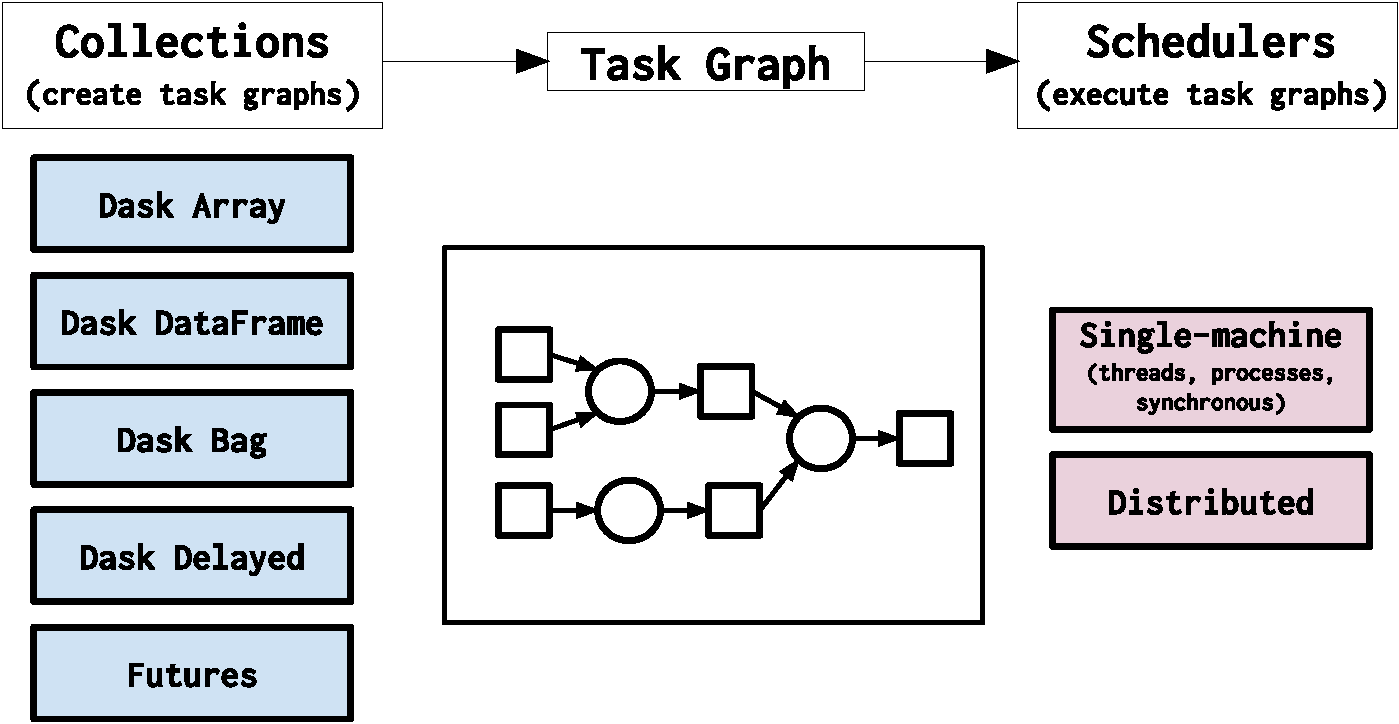
\includegraphics[width=.75\textwidth]{pic/dask-overview}
    \caption{Dask functionality \cite{daskhomepage2020}}
    \label{fig:dask-overview}
\end{figure}



Dask \cite{daskhomepage2020} is a flexible library for parallel computing in Python.
It is composed of these parts:
\begin{enumerate}
\item Scheduler: Dynamic task scheduling optimized for computation. This is similar to Airflow, Luigi, Celery, or Make, but optimized for interactive computational workloads.
\item Graphs: Dask represents parallel computations with task graphs.  Working directly with dask graphs is rare, unless you intend to develop new modules with Dask. Dask graphs are created internally and most users don't ever see a graph. See Section~\ref{sec:DaskComputeGraphs} for an example of a Dask graph.
\item Collections: ``Big Data'' collections like parallel arrays, dataframes, and lists that extend common interfaces like NumPy, Pandas, or Python iterators to larger-than-memory or distributed environments. These parallel collections run on top of dynamic task schedulers.
\end{enumerate}

The graph and collections functionalities are very powerful but not used in the \libradtrandask{} module. These topics are not further considered here.

Dask installs  conveniently  on a laptop, a desktop or a cluster computer. Dask can scale to a cluster of 100s of machines. This ease of transition between single-machine to moderate cluster enables users to both start simple and grow when necessary.  The \libradtrandask{} module uses the Dask scheduler to run \libradtran{} on a Linux computer, serving locally or to remote computers.

\section{Dask as Server}

The client Client-Server design pattern is generally used in the context where any number of clients, running on many different (weaker) computers can access the centralised server that is highly optimised to perform a specific set of functions very efficiently.  A common instance of this pattern is in enterprise database systems such as SAP or PeopleSoft. The clients have a small footprint (called 'thin', perhaps even just a browser), with most of the functionality in the main server (often with big databases and high processing capability).

A cloud service is any service made available to users on demand via the Internet from a cloud computing provider's servers as opposed to being provided from a company's own on-premises servers. Cloud services are designed to provide easy, scalable access to applications, resources and services, and are fully managed by a cloud services provider.
In the context of this document, consider the cloud service as a massively parallel computer providing computing and/or storage via the internet.

Dask is neither of the above, it is a technology that enables parallel computation, either on the local computer, on other computers on a private network or even in a cloud service.
Using the Dask distributed module a server-like functionality can be implemented  for doing remote processing in a specialist area --- this is what the current application is doing.

Setting up a distributed computation server with Dask requires that work on the local PC and work on the server be done in Python. Even more strictly, exactly the same versions of Python and all required modules must be installed on all computers.  This requirement stems from Dask's packaging (using pickle or dill) of the code to be executed as well as the data to be used. The combined package of code and data is sent to the remote computer, which returns the resulting data after computation. This model is fundamentally different from conventional servers.

\section{Dask \lstinlineL{Distributed}}



\begin{figure}[htbp]
    \centering
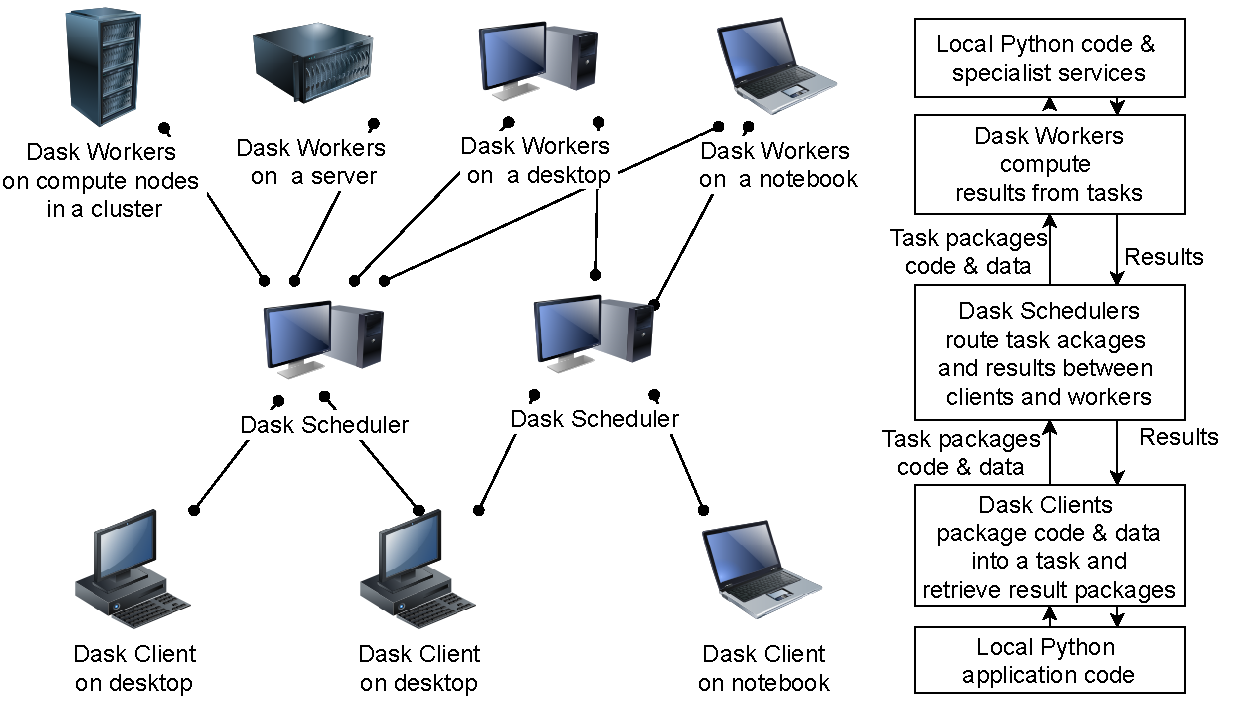
\includegraphics[width=\textwidth]{pic/dask-scheduler}
    \caption{Dask distributed concept}
    \label{fig:dask-scheduler}
\end{figure}

The Dask distributed concept has three major roles:
\begin{enumerate}
    \item Clients: The client resides on a local PC (of any form) which puts together a package of code and data. This package is pickled\footnote{Pickle is a Python way to serialise complex objects into a single package.} and sent to a scheduler.  The client also receives results back from the scheduler. So the client sends task packages and retrieves results.  There can be any number of clients, on any number of computers. One client can communicate with any number of schedulers.

    \item Schedulers: The scheduler listens on a specific port for any client requests. At the same time, the scheduler also polls the workers to keep record of `idle' workers that are available to take on new tasks.  Task packages from clients are routed to available workers for execution. When the worker has completed the task, the scheduler can make it available when the client requests the results. There can be any number of schedulers, on any number of computers. One scheduler can communicate with any number of clients and any number of workers.

    \item Workers: The workers wait for task assignments from the scheduler. When the task package is received it is executed on the worker node CPU. The results are packaged and stored until retrieved by the scheduler.   There can be any number of workers, on any number of computing nodes or computers. One worker can communicate with any number of schedulers.
\end{enumerate}



\begin{figure}[htbp]
    \centering
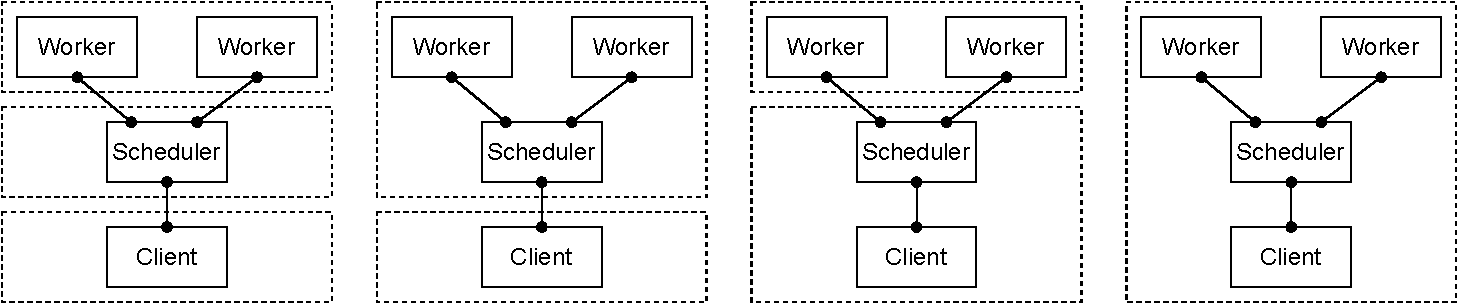
\includegraphics[width=\textwidth]{pic/daskdistriballoc}
    \caption[Dask distributed in different computers configurations]{Dask distributed in different computers configurations. The dotted lines represent different computers}
    \label{fig:daskdistriballoc}
\end{figure}

The Client, the Scheduler and the Worker are all independently running code instances, which could be running on one or more computers. Figure~\ref{fig:daskdistriballoc} shows the options for running the processes. The figure shows the computer hardware boundaries in dashed lines. It is evident that the different processes can run on the same computer, different computers or any mix of computers.  Each computer is identified by an IP address on the network and the network location (IP addresses) of the scheduler and worker computers are specified in the code. Hence, the IP addresses must be known before the code is executed.


\section{Executing User Code}

How does this Dask Distributed fit into the user code?
Imagine the scenario where a Windows user requires a \libradtran{} run, but does not have it compiled for his Windows PC.  Suppose \libradtran{} is available on a Linux computer somewhere on the network. The Linux computer can be single computer in the office next door, or it can be a server on the local network or even in a cloud service.

The user Python application sets up a task package containing some Python code to run \libradtran{} on the remote computer and the input files for the run. The package and execution proceeds from user application code to the Dask client on the local PC, to the scheduler, to the worker (the worker then does some work on the data), the results are then sent back to the scheduler, back to the client, and finally back to the  user code, where the results are processed.  This process can be followed for  a single \libradtran{} run or it can be for thousands of runs, where each run is executed on one of many different workers.  The workers run concurrently on a cluster or on multiple cores in a local CPU.

Once the Dask distributed channel is set up, the user has no further action than to set up the task package.  The distribution and execution is all taken care of by Dask.  The price to be paid for this convenience is setting up the scheduler and worked environments, which is relatively small.  Of course, setting up \libradtran{}  must be done anyway, either on the local or remote computer, so there is no penalty here. In fact, building \libradtran{}  on a Linux PC is relatively simple and quick.

How does the worker know what processing is required?
The package delivered to the worker contains Python code and the input data.
The worker simply executes the Python code in the package, on the data in the package.
The package code can be only Python code, such as a Python machine learning algorithm, but the Python code can also execute other executable codes (such as \libradtran{}) on the worker node. The process to execute other codes will be described later in this report.

\section{Serialisation}

\begin{figure}[htbp]
    \centering
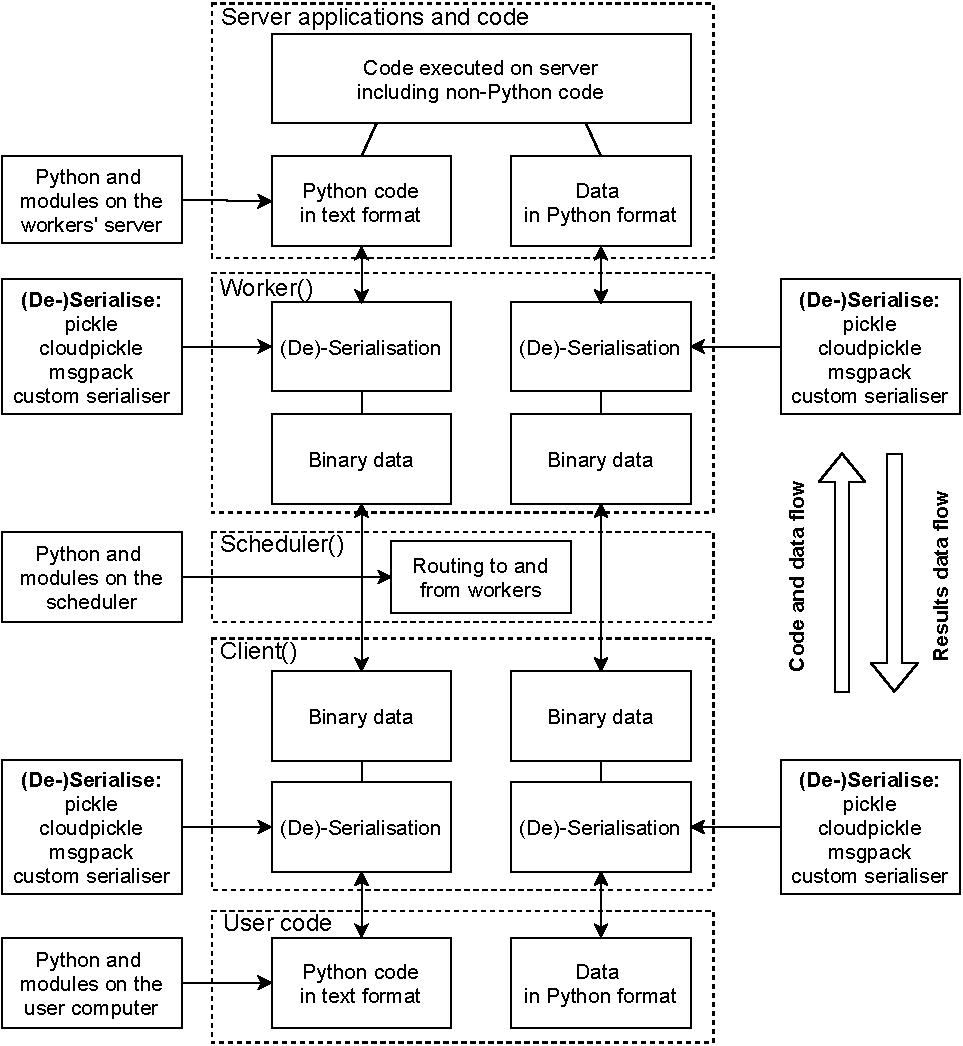
\includegraphics[width=\textwidth]{pic/DaskSerialisation}
    \caption{Dask serialisation}
    \label{fig:DaskSerialisation}
\end{figure}

Passing data between computers requires conversion of the data into a sequence of bytes that can be communicated across the network. The code and data flowing from the user PC to the scheduler and worker must be 'zipped-up'\footnote{The term zip up is used figuratively, it is not implying that the pkzip technology is used.} into a package. This is called serialisation.
Choices made in serialization can affect performance and security.
Dask serialisation is described here: 
\lstinlineN{https://distributed.dask.org/en/latest/serialization.html}.

The standard Python solution to this, Pickle, is often but not always the right solution. Dask uses a number of different serialization schemes in different situations. These are extensible to allow users to control in sensitive situations and also to enable library developers to plug in higher performing serialization solutions. Figure~\ref{fig:DaskSerialisation} shows the serialisation process in Dask.


There are three kinds of messages passed through the Dask network:

\begin{enumerate}
    \item Small administrative messages like ``Worker A has finished task X'' or ``I'm running out of memory''. These are always serialized with \lstinlineN{msgpack}.
    \item  Movement of program data, such as Numpy arrays and Pandas dataframes. This uses a combination of pickle, cloudpickle, msgpack, and custom per-type serialisers that come with Dask.
    \item Computational tasks (Python code) like \lstinlineN{f(x)} that are defined and serialized on client processes and deserialized and run on worker processes. These are serialized using a fixed scheme decided on by those libraries. Today this is a combination of pickle and cloudpickle.

\end{enumerate}
You can choose which families you want to use to serialize data and to deserialize data when you create a client.

The various serialisation modules implement compact binary protocols for serializing and de-serializing a Python object structure. These protocols are unique and version specific, which may lead to incompatibilities between the serialised data and the module versions used to deserialise the data. Most of these serialisation module formats are not transportable between versions.

For more information on the pickle module see \\
\lstinlineN{https://docs.python.org/3/library/pickle.html}, and \\
\lstinlineN{https://docs.python.org/2/library/pickle.html}.


\section{Versions}

Careful review of Figure~\ref{fig:DaskSerialisation} indicates that there are potentially three different Python instances: one each in the user computer, the scheduler computer and one in the worker computer\footnote{If all three instances are on the same computer then the same Python is used.}.  The way Dask works is to pass the Python code for execution to the other computer. If these versions differ, there could be complications.  The idea is that the code should execute exactly the same irrespective of which computer it is executed on. Hence the software versions of Python and all the modules used, must be exactly the same on all computers --- even to the bug fix version (the last number in the three-number version number).

Dask should check the versions as default action when the packages are sent around. If the versions are different the user is warned and the processes is stopped. 
If the versions do not match an error report similar to the following may be displayed. 
The Dask software is continuously updated so the format may differ from as it is shown here.

\begin{lstlisting}
distributed.worker - WARNING - Mismatched versions found

distributed
+---------------------------+---------------------------+
|                           | version                   |
+---------------------------+---------------------------+
| This Worker               | 2.11.0+21.g05ca3fb1.dirty |
| scheduler                 | 2.12.0                    |
| tcp://192.168.0.102:64357 | 2.11.0+21.g05ca3fb1.dirty |
+---------------------------+---------------------------+

msgpack
+---------------------------+---------+
|                           | version |
+---------------------------+---------+
| This Worker               | 0.6.1   |
| scheduler                 | 1.0.0   |
| tcp://192.168.0.102:64357 | 0.6.1   |
+---------------------------+---------+
\end{lstlisting}

or 

\begin{lstlisting}
ValueError: Mismatched versions found

cloudpickle
+------------------------+---------+
|                        | version |
+------------------------+---------+
| client                 | 0.5.3   |
| scheduler              | 0.5.2   |
| tcp://100.96.1.5:36964 | 0.5.2   |
| tcp://100.96.1.6:38415 | 0.5.2   |
| tcp://100.96.2.6:44389 | 0.5.2   |
| tcp://100.96.2.7:39214 | 0.5.2   |
| tcp://100.96.2.8:40317 | 0.5.2   |
+------------------------+---------+

dask
+------------------------+---------+
|                        | version |
+------------------------+---------+
| client                 | 0.18.2  |
| scheduler              | 0.17.4  |
| tcp://100.96.1.5:36964 | 0.17.4  |
| tcp://100.96.1.6:38415 | 0.17.4  |
| tcp://100.96.2.6:44389 | 0.17.4  |
| tcp://100.96.2.7:39214 | 0.17.4  |
| tcp://100.96.2.8:40317 | 0.17.4  |
+------------------------+---------+
\end{lstlisting}

If the process does not work correctly, check for the versions by using \\
\lstinlineN{client.get_versions(check=True)},\\
 that returns the current versions in a json file.

\begin{lstlisting}
{'scheduler': {'host': (('python', '3.7.6.final.0'),
   ('python-bits', 64),
   ('OS', 'Windows'),
   ('OS-release', '7'),
   ('machine', 'AMD64'),
   ('processor', 'Intel64 Family 6 Model 94 Stepping 3, GenuineIntel'),
   ('byteorder', 'little'),
   ('LC_ALL', 'None'),
   ('LANG', 'None')),
  'packages': {'dask': '2.12.0',
   'distributed': '2.12.0',
   'msgpack': '0.6.1',
   'cloudpickle': '1.3.0',
   'tornado': '6.0.4',
   'toolz': '0.10.0',
   'numpy': '1.18.1',
   'lz4': None,
   'blosc': None}},
 'workers': {'tcp://127.0.0.1:63694': {'host': (('python', '3.7.6.final.0'),
    ('python-bits', 64),
    ('OS', 'Windows'),
    ('OS-release', '7'),
    ('machine', 'AMD64'),
    ('processor', 'Intel64 Family 6 Model 94 Stepping 3, GenuineIntel'),
    ('byteorder', 'little'),
    ('LC_ALL', 'None'),
    ('LANG', 'None')),
   'packages': {'dask': '2.12.0',
    'distributed': '2.12.0',
    'msgpack': '0.6.1',
    'cloudpickle': '1.3.0',
    'tornado': '6.0.4',
    'toolz': '0.10.0',
    'numpy': '1.18.1',
    'lz4': None,
    'blosc': None}}},
 'client': {'host': [('python', '3.7.6.final.0'),
   ('python-bits', 64),
   ('OS', 'Windows'),
   ('OS-release', '7'),
   ('machine', 'AMD64'),
   ('processor', 'Intel64 Family 6 Model 94 Stepping 3, GenuineIntel'),
   ('byteorder', 'little'),
   ('LC_ALL', 'None'),
   ('LANG', 'None')],
  'packages': {'dask': '2.12.0',
   'distributed': '2.12.0',
   'msgpack': '0.6.1',
   'cloudpickle': '1.3.0',
   'tornado': '6.0.4',
   'toolz': '0.10.0',
   'numpy': '1.18.1',
   'lz4': None,
   'blosc': None}}}
\end{lstlisting}

The solution to this problem is to ensure that the same versions are present on all computers.
See Section~\ref{sec:Additionalpackages} on installing specific package versions.




\section{Dask Experiments}
\label{sec:DaskExperiments}

The rest of this chapter is an extract from this notebook:\\
\lstinline{https://github.com/NelisW/miscellania/blob/master/dask/Dask-Experiments.ipynb}


\subsection{Setting Up}
\label{sec:SettingUp}

The following page explain in more detail how to set up Dask on a variety of local and distributed hardware.
\lstinline{https://docs.dask.org/en/latest/setup.html}


There are two ways to set up Dask on a local computer. Both of these ways are explored in the notebook.
Setting up on a local computer is important to grasp the concepts even if the end objective is to use a multi PC configuration.


There are several multi-computer set up techniques. This document explores two techniques: manual set up and SSH set up.



\begin{lstlisting}[style=incellstyle]
from dask.distributed import Client, LocalCluster

\end{lstlisting}


\subsection{Single Machine (local PC)}
\label{sec:SingleMachinelocalPC}

The \verb+dask.distributed+ scheduler works well on a single machine. It is sometimes preferred over the default scheduler. 
You can create a \verb+dask.distributed+ scheduler by importing and creating a Client with no arguments. This overrides whatever default was previously set.  In the context of this section, the word distributed is understood to be distributed programmatically on the local physical computer (not distributed in the physical sense).


The \verb+Client()+ call used here  is shorthand for creating a \verb+LocalCluster+ and then passing that to your client.
You may want to look at the wider range  keyword arguments available on \verb+LocalCluster+ to understand the options available to you on handling the mixture of threads and processes, like specifying explicit ports, and so on. For example, if you use the \verb+localCluster+ approach you can set the number of workers.


Note that \verb+Client()+ and \verb+LocalCluster()+ take many optional arguments, to configure the server.


You can navigate to \verb+http://localhost:8787/status+ to see the diagnostic dashboard if you have Bokeh installed.


Once the local client is started it will start a local cluster, but all working on the local computer.


The \verb+client.scheduler\_info()+ command provides information about the client, server and worker setup.


The \verb+client.shutdown()+ command can be used to shut down the client on the server


\lstinline{https://docs.dask.org/en/latest/setup/single-distributed.html }


\lstinline{https://distributed.dask.org/en/latest/api.html#distributed.Client}


Dask is not the only means to do parallel processing.  See also this tutorial on multiprocessing.


\lstinline{https://sebastianraschka.com/Articles/2014\_multiprocessing.html}



\begin{lstlisting}[style=incellstyle]
# to use use local host
useSimpleClient = True

if useSimpleClient:
    # simplified setup, less control
    client = Client() 
else:
    # Setup a local cluster, more control
    # By default this sets up 1 worker per core    
    cluster = LocalCluster(n_workers=1)
    client = Client(cluster)

client.get_versions(check=True)

client
\end{lstlisting}

\begin{center}

\begin{normalsize}

\begin{tabular}{|c|c|}
\hline
Client

  Scheduler: tcp://127.0.0.1:64865
  Dashboard: http://127.0.0.1:8787/status&Cluster

  Workers: 4
  Cores: 8
  Memory: 34.00 GB\\\hline

\end{tabular}
\end{normalsize}
\end{center}


\begin{lstlisting}[style=incellstyle]
client.scheduler_info()
\end{lstlisting}


\begin{lstlisting}[style=outcellstyle]
{'type': 'Scheduler',
 'id': 'Scheduler-e40d7349-ee4d-481f-b416-bc9b75b87b92',
 'address': 'tcp://127.0.0.1:64865',
 'services': {'dashboard': 8787},
 'workers': {'tcp://127.0.0.1:64887': {'type': 'Worker',
   'id': 3,
   'host': '127.0.0.1',
   'resources': {},
   'local_directory': 'V:\\work\\WorkN\\miscellania\\dask\\dask-worker-space\\worker-sz1aoteq',
   'name': 3,
   'nthreads': 2,
   'memory_limit': 8500740096,
   'last_seen': 1586869485.3058014,
   'services': {},
   'metrics': {'cpu': 0.0,
    'memory': 52654080,
    'time': 1586869485.2592325,
    'read_bytes': 0.0,
    'write_bytes': 0.0,
    'executing': 0,
    'in_memory': 0,
    'ready': 0,
    'in_flight': 0,
    'bandwidth': {'total': 100000000, 'workers': {}, 'types': {}}},
   'nanny': 'tcp://127.0.0.1:64868'},
  'tcp://127.0.0.1:64889': {'type': 'Worker',
   'id': 2,
   'host': '127.0.0.1',
   'resources': {},
   'local_directory': 'V:\\work\\WorkN\\miscellania\\dask\\dask-worker-space\\worker-a3868zvm',
   'name': 2,
   'nthreads': 2,
   'memory_limit': 8500740096,
   'last_seen': 1586869485.3589983,
   'services': {},
   'metrics': {'cpu': 0.0,
    'memory': 52600832,
    'time': 1586869485.3125384,
    'read_bytes': 0.0,
    'write_bytes': 0.0,
    'executing': 0,
    'in_memory': 0,
    'ready': 0,
    'in_flight': 0,
    'bandwidth': {'total': 100000000, 'workers': {}, 'types': {}}},
   'nanny': 'tcp://127.0.0.1:64870'},
  'tcp://127.0.0.1:64890': {'type': 'Worker',
   'id': 1,
   'host': '127.0.0.1',
   'resources': {},
   'local_directory': 'V:\\work\\WorkN\\miscellania\\dask\\dask-worker-space\\worker-jou7s9bk',
   'name': 1,
   'nthreads': 2,
   'memory_limit': 8500740096,
   'last_seen': 1586869485.3625963,
   'services': {},
   'metrics': {'cpu': 0.0,
    'memory': 52740096,
    'time': 1586869485.3174865,
    'read_bytes': 0.0,
    'write_bytes': 0.0,
    'executing': 0,
    'in_memory': 0,
    'ready': 0,
    'in_flight': 0,
    'bandwidth': {'total': 100000000, 'workers': {}, 'types': {}}},
   'nanny': 'tcp://127.0.0.1:64869'},
  'tcp://127.0.0.1:64893': {'type': 'Worker',
   'id': 0,
   'host': '127.0.0.1',
   'resources': {},
   'local_directory': 'V:\\work\\WorkN\\miscellania\\dask\\dask-worker-space\\worker-djqrx1np',
   'name': 0,
   'nthreads': 2,
   'memory_limit': 8500740096,
   'last_seen': 1586869485.4007897,
   'services': {},
   'metrics': {'cpu': 0.0,
    'memory': 52621312,
    'time': 1586869485.3620787,
    'read_bytes': 0.0,
    'write_bytes': 0.0,
    'executing': 0,
    'in_memory': 0,
    'ready': 0,
    'in_flight': 0,
    'bandwidth': {'total': 100000000, 'workers': {}, 'types': {}}},
   'nanny': 'tcp://127.0.0.1:64867'}}}
\end{lstlisting}


\begin{lstlisting}[style=incellstyle]
# client.shutdown()
\end{lstlisting}


\begin{lstlisting}[style=incellstyle]
#client.get_versions(check=True)
\end{lstlisting}

There are a few different ways to interact with the cluster through the client:


\begin{enumerate}
\item The Client satisfies most of the standard concurrent.futures - PEP-3148 interface with \verb+.submit+, \verb+.map+ functions and \verb+Future+ objects, allowing the immediate and direct submission of tasks \lstinline{https://docs.python.org/3/library/concurrent.futures.html}.
\item The Client registers itself as the default Dask scheduler, and so runs all dask collections like \verb+dask.array+, \verb+dask.bag+, \verb+dask.dataframe+ and \verb+dask.delayed+
\item The Client has additional methods for manipulating data remotely. See the full API for a thorough list \lstinline{https://distributed.dask.org/en/latest/api.html}.
\end{enumerate}


\subsubsection{Dask Dashboard}
\label{sec:DaskDashboard}

The Dask dashboard is a bokeh-based display of what is taking place in the server and its workers. For this to work the Python bokeh package must be installed.


Workers capture durations associated to tasks. For each task that passes through a worker we record start and stop times for each of the following:


\begin{itemize}
\item Serialization (gray)
\item Dependency gathering from peers (red)
\item Disk I/O to collect local data (orange)
\item Execution times (colored by task)
\end{itemize}

The main way to observe these times is with the task stream plot on the scheduler's /status page where the colors of the bars correspond to the colors listed above.


\lstinline{https://docs.dask.org/en/latest/diagnostics-distributed.html}


\lstinline{https://distributed.dask.org/en/latest/diagnosing-performance.html}


\lstinline{https://medium.com/@kartikbhanot/dask-scheduler-dashboard-understanding-resource-and-task-allocation-in-local-machines-bc5aa60eca6e}


\lstinline{https://www.youtube.com/watch?v=N\_GqzcuGLCY}


There is also a Dask extension for Jupyter notebooks \verb+dask-labextension+.


\lstinline{https://github.com/dask/dask-labextension}



\begin{lstlisting}[style=incellstyle]
# to obtain the dashboard for the client
def clientDashboardURI(client):
    """Extract the bokeh dashboard URI from the client's scheduler info
    """
    
    dashboardURI = client.scheduler_info()['address'].rsplit(':',1)[0]+':'
    dashboardURI += str(client.scheduler_info()['services']['dashboard'])
    
    return dashboardURI.replace('tcp:','http:')

print(clientDashboardURI(client))
\end{lstlisting}


\begin{lstlisting}[style=outcellstyle]
http://127.0.0.1:8787

\end{lstlisting}

Open a browser window with the above URI (for the currently running client). Set the \verb+if+ condition to \verb+True+ and execute the code below to observe the dashboard in action.
The code below is not meaningful it is just meant to keep Dask busy for a while.


While the code is executing, click on the different tabs in the dashboard to learn about the different displays.



\begin{lstlisting}[style=incellstyle]
if False:
    import dask.array as da
    x = da.random.random((10000, 10000,10), chunks=(1000,1000,5))
    y = da.random.random((10000, 10000,10), chunks=(1000,1000,5))
    z = (da.arcsin(x)+da.arccos(y)).sum(axis=(1,2))
    z.compute()
\end{lstlisting}


\subsubsection{Preparing functions}
\label{sec:Preparingfunctions}

Create a few functions that will be used in the examples.



\begin{lstlisting}[style=incellstyle]
# to create simple task to experiment with
def inc(x):
    return x + 1

def add(x, y):
    return x + y

\end{lstlisting}


\subsubsection{Single function calls}
\label{sec:Singlefunctioncalls}

Using the client created above, a single function and a single data (datum?) item will be dispatched to the scheduler and worker. All of the scheduling work is transparent.


We can submit individual function calls with the \verb+client.submit+ method.


The simple example here will execute much faster in normal in-line Python code, the idea here is to show the Dask method.


The \verb+submit+ function returns a \verb+Future+, which refers to a (future) remote result. This result may not yet be completed. Eventually it will complete. The result stays in the remote thread/process/worker until you ask for it back explicitly by calling the \verb+result+ method on the future itself (not a client method as for the map case below).


\lstinline{https://distributed.dask.org/en/latest/client.html}



\begin{lstlisting}[style=incellstyle]
# to create a single future
x1 = client.submit(inc, 10)
print(x1)
\end{lstlisting}


\begin{lstlisting}[style=outcellstyle]
<Future: pending, key: inc-083b5e2ba45c380966bcb963d4544e5e>

\end{lstlisting}


\begin{lstlisting}[style=incellstyle]
# to see what a future looks like
print(x1)
\end{lstlisting}


\begin{lstlisting}[style=outcellstyle]
<Future: finished, type: builtins.int, key: inc-083b5e2ba45c380966bcb963d4544e5e>

\end{lstlisting}


\begin{lstlisting}[style=incellstyle]
# to retrieve a result from a future
x1r = x1.result()
print(x1r)
\end{lstlisting}


\begin{lstlisting}[style=outcellstyle]
11

\end{lstlisting}


\begin{lstlisting}[style=incellstyle]
# to check if a future resets or disappears after its initial retrieval
print(x1)
x1r = x1.result()
print(x1r)
\end{lstlisting}


\begin{lstlisting}[style=outcellstyle]
<Future: finished, type: builtins.int, key: inc-083b5e2ba45c380966bcb963d4544e5e>
11

\end{lstlisting}

You can pass futures as inputs to submit. Dask automatically handles dependency tracking; once all input futures have completed, they will be moved onto a single worker (if necessary), and then the computation that depends on them will be started. You do not need to wait for inputs to finish before submitting a new task; Dask will handle this automatically:



\begin{lstlisting}[style=incellstyle]
# to create a graph of futures
x1 = client.submit(inc, 10)
x2 = client.submit(inc, 10)
print(x1)
print(x2)
xs = client.submit(add,x1,x2)
print(xs)
\end{lstlisting}


\begin{lstlisting}[style=outcellstyle]
<Future: finished, type: builtins.int, key: inc-083b5e2ba45c380966bcb963d4544e5e>
<Future: finished, type: builtins.int, key: inc-083b5e2ba45c380966bcb963d4544e5e>
<Future: pending, key: add-6e6cf98db4b0523bbdc831467bd5720b>

\end{lstlisting}


\begin{lstlisting}[style=incellstyle]
# to print the result of the graph final output
xsr = xs.result()
print(xsr)
\end{lstlisting}


\begin{lstlisting}[style=outcellstyle]
22

\end{lstlisting}


\subsubsection{Multiple function calls}
\label{sec:Multiplefunctioncalls}

Using the client created above, a single function and multiple data items will be dispatched to the scheduler and worker. All of the scheduling work is transparent.


Similar to Python's \verb+map+, you can use \verb+Client.map+ to call the same function and many inputs.


The returns a list of futures.
These results live on the distributed workers.


We can submit tasks on futures. The function will go to the machine where the futures are stored and run on the result once it has completed.In the example below the list of futures is sent to the built-in Python \verb+sum()+ function, which adds the elements of an iterable and returns the sum.



\begin{lstlisting}[style=incellstyle]
# to create a map of input values for a function
futures  = client.map(inc, [2, 4, 6])
for future in futures:
    print(future)
\end{lstlisting}


\begin{lstlisting}[style=outcellstyle]
<Future: pending, key: inc-423e89f2660795305fd6c03c55d1de5d>
<Future: pending, key: inc-98feef5b8b4598158d0e47a6d4acde9d>
<Future: pending, key: inc-d016ddc28876119154a07cfbe98a9ed7>

\end{lstlisting}

The results stay in the remote thread/process/worker until you ask for it back explicitly by calling the client \verb+gather+ method (not the future's result method) because here a list must be processed.



\begin{lstlisting}[style=incellstyle]
# to gather the list of results
futuresr = client.gather(futures)
print(futuresr)
\end{lstlisting}


\begin{lstlisting}[style=outcellstyle]
[3, 5, 7]

\end{lstlisting}


\begin{lstlisting}[style=incellstyle]
# to graph a list of futures into another submit
total = client.submit(sum, futures)
print(total)
 
totalr = total.result()
print(totalr)
\end{lstlisting}


\begin{lstlisting}[style=outcellstyle]
<Future: pending, key: sum-c34d59da0efacac3f60627d03084e274>
15

\end{lstlisting}

\subsubsection{Serialising Code and Data}
\label{sec:SerialisingCodeandData}

In the examples shown above the code and data are serialised in the client before passing on to the scheduler. This can be visualised as shown in Figure~\ref{fig:DaskSerialisation02}.


\begin{figure}[htbp]
    \centering
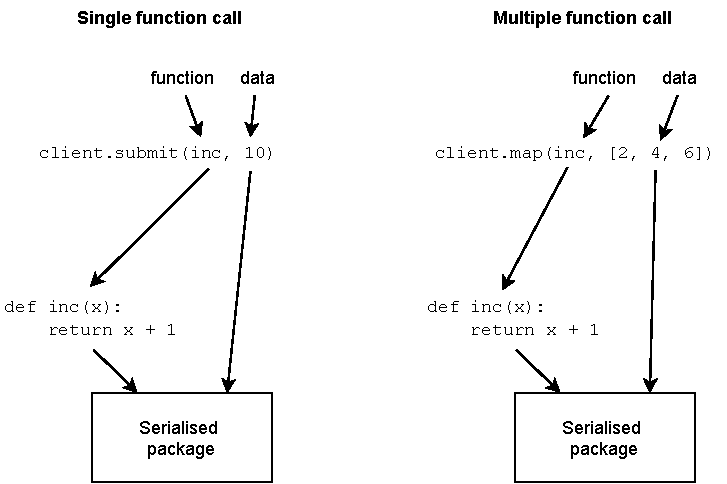
\includegraphics[width=.8\textwidth]{pic/DaskSerialisation02}
    \caption{Dask serialisation and worker execution visualised}
    \label{fig:DaskSerialisation02}
\end{figure}


\subsection{Multiple Machines (local PC and Remote Server(s))}
\label{sec:MultipleMachineslocalPCandRemoteServers}


\subsubsection{Setting up}
\label{sec:Settingup}

For the sake of these discussions suppose the computers have the following  IP addresses (replace with the IP addresses on your system):
\begin{enumerate}
\item Local computer running the \verb+dask.distributed.Client+:  \verb+146.64.202.163+
\item Computer running the scheduler: \verb+146.64.246.94+
\item Computer running the workers: \verb+146.64.246.94+
\end{enumerate}



In this case the scheduler and worker are run on the same server, but could be ran on different computers.


All three computers must have exactly the same versions of Python, dask, pickle, etc., otherwise the following will not work. If required versions are available in a Python environment, the environment must be activated.


The client, scheduler and workers must be able to communicate with each other. This is achieved by using selected ports and IP addresses. The main IP address of interest here is the scheduler IP address which must be made known to the client and the workers, see the example below.

\begin{figure}[htbp]
    \centering
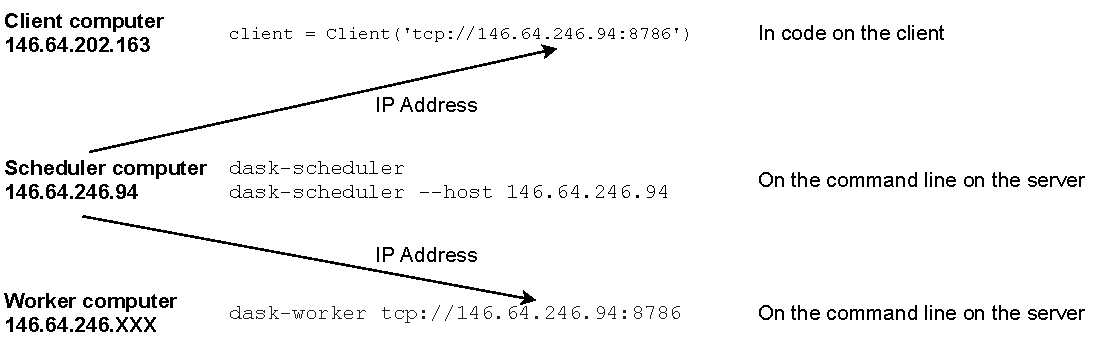
\includegraphics[width=\textwidth]{pic/serverIP}
    \caption{IP port notification in Dask}
    \label{fig:serverIP}
\end{figure}


Start the scheduler and workers:


\begin{enumerate}
\item \textbf{Start the scheduler on the server}. Log in to the server (\lstinline{146.64.246.94}), then activate the Python environment and start the scheduler:

\begin{lstlisting}
conda activate devpy37
dask-scheduler
\end{lstlisting}

If the server already has the necessary Python, dask and pickle versions in the root Python environment there is no need to first activate the Python environment.  In this case the scheduler can be started from any computer by specifying the hostname. So on the local computer the following command will start the scheduler (if versions are correct in the root Python):

\begin{lstlisting}
dask-scheduler --host 146.64.246.94
\end{lstlisting}

Either of the above should start the scheduler:
\begin{lstlisting}[style=tinysize]
(devpy37) username@servername:~$ dask-scheduler
 distributed.scheduler - INFO - -----------------------------------------------
 distributed.scheduler - INFO - Local Directory:    /tmp/scheduler-mxiy5sli
 distributed.scheduler - INFO - -----------------------------------------------
 distributed.scheduler - INFO - Clear task state
 distributed.scheduler - INFO -   Scheduler at:  tcp://146.64.246.94:8786
 distributed.scheduler - INFO -   dashboard at:                     :8787
 distributed.scheduler - INFO - Register worker <Worker 'tcp://146.64.246.94:45347', name: tcp://146.64.246.94:45347, memory: 0, processing: 0>
 distributed.scheduler - INFO - Starting worker compute stream, tcp://146.64.246.94:45347
 distributed.core - INFO - Starting established connection
\end{lstlisting}

\item \textbf{Start the worker on the server}  Log in to the server (\lstinline{146.64.246.94}), then activate the Python environment and start the worker:        

\begin{lstlisting}
dask-worker tcp://146.64.246.94:8786
\end{lstlisting}

where the IP address and port number must correspond to the scheduler IP and port address. This should start the worker task. Note that the dashboard IP address is also given when the workers start. This server has 32 cores and 32 GB memory.    

\begin{lstlisting}[style=tinysize]
(devpy37) username@servername:~$ dask-worker tcp://146.64.246.94:8786
distributed.nanny - INFO -         Start Nanny at: 'tcp://146.64.246.94:35459'
distributed.worker - INFO -       Start worker at:  tcp://146.64.246.94:45347
distributed.worker - INFO -          Listening to:  tcp://146.64.246.94:45347
distributed.worker - INFO -          dashboard at:        146.64.246.94:42791
distributed.worker - INFO - Waiting to connect to:   tcp://146.64.246.94:8786
distributed.worker - INFO - -------------------------------------------------
distributed.worker - INFO -               Threads:                         32
distributed.worker - INFO -                Memory:                   33.71 GB
distributed.worker - INFO -       Local Directory: /home/username/dask-worker-space/worker-lz08iq0s
distributed.worker - INFO - -------------------------------------------------
distributed.worker - INFO -         Registered to:   tcp://146.64.246.94:8786
distributed.worker - INFO - -------------------------------------------------
distributed.core - INFO - Starting established connection
\end{lstlisting}

\item \textbf{Start the client}  When the client is initiated, pass the scheduler IP:port address:

\begin{lstlisting}[style=tinysize]
# to start a local client with a remote scheduler
client = Client('146.64.246.94:8786') 
\end{lstlisting}

To see the Python module versions:
\begin{lstlisting}[style=tinysize]
client.get_versions(check=True)
\end{lstlisting}

\begin{lstlisting}[style=outcellstyle]
{'scheduler': {'host': (('python', '3.7.6.final.0'),
   ('python-bits', 64),
   ('OS', 'Linux'),
   ('OS-release', '4.9.0-8-amd64'),
   ('machine', 'x86_64'),
   ('processor', ''),
   ('byteorder', 'little'),
   ('LC_ALL', 'None'),
   ('LANG', 'en_ZA.UTF-8')),
  'packages': {'dask': '2.12.0',
   'distributed': '2.12.0',
   'msgpack': '0.6.1',
   'cloudpickle': '1.3.0',
   'tornado': '6.0.4',
   'toolz': '0.10.0',
   'numpy': '1.18.1',
   'lz4': None,
   'blosc': None}},
 'workers': {'tcp://146.64.246.94:45347': {'host': (('python',
     '3.7.6.final.0'),
    ('python-bits', 64),
    ('OS', 'Linux'),
    ('OS-release', '4.9.0-8-amd64'),
    ('machine', 'x86_64'),
    ('processor', ''),
    ('byteorder', 'little'),
    ('LC_ALL', 'None'),
    ('LANG', 'en_ZA.UTF-8')),
   'packages': {'dask': '2.12.0',
    'distributed': '2.12.0',
    'msgpack': '0.6.1',
    'cloudpickle': '1.3.0',
    'tornado': '6.0.4',
    'toolz': '0.10.0',
    'numpy': '1.18.1',
    'lz4': None,
    'blosc': None}}},
 'client': {'host': [('python', '3.7.6.final.0'),
   ('python-bits', 64),
   ('OS', 'Windows'),
   ('OS-release', '7'),
   ('machine', 'AMD64'),
   ('processor', 'Intel64 Family 6 Model 94 Stepping 3, GenuineIntel'),
   ('byteorder', 'little'),
   ('LC_ALL', 'None'),
   ('LANG', 'None')],
  'packages': {'dask': '2.12.0',
   'distributed': '2.12.0',
   'msgpack': '0.6.1',
   'cloudpickle': '1.3.0',
   'tornado': '6.0.4',
   'toolz': '0.10.0',
   'numpy': '1.18.1',
   'lz4': None,
   'blosc': None}}}
\end{lstlisting}

To see the Dask scheduler information:
\begin{lstlisting}[style=tinysize]
client.scheduler_info()
\end{lstlisting}

\begin{lstlisting}[style=outcellstyle]
{'type': 'Scheduler',
 'id': 'Scheduler-c18c6181-421b-4826-aea7-b1bba21efeb0',
 'address': 'tcp://146.64.246.94:8786',
 'services': {'dashboard': 8787},
 'workers': {'tcp://146.64.246.94:45347': {'type': 'Worker',
   'id': 'tcp://146.64.246.94:45347',
   'host': '146.64.246.94',
   'resources': {},
   'local_directory': '/home/dgriffith/dask-worker-space/worker-lz08iq0s',
   'name': 'tcp://146.64.246.94:45347',
   'nthreads': 32,
   'memory_limit': 33712070656,
   'last_seen': 1586869487.8488212,
   'services': {'dashboard': 42791},
   'metrics': {'cpu': 2.0,
    'memory': 107896832,
    'time': 1586869487.3504004,
    'read_bytes': 16650.21565100753,
    'write_bytes': 1014.9159528091943,
    'num_fds': 25,
    'executing': 0,
    'in_memory': 0,
    'ready': 0,
    'in_flight': 0,
    'bandwidth': {'total': 100000000, 'workers': {}, 'types': {}}},
   'nanny': 'tcp://146.64.246.94:35459'}}}
\end{lstlisting}

\end{enumerate}



\subsubsection{Running workers remotely}
\label{sec:Runningworkersremotely}

Now execute the same graph as on the single computer before, but now on the remote server.


To see if the server is running, put the \verb+client()+ call in a Python exception.



\begin{lstlisting}[style=incellstyle]
# to run the graph on a remove server

try:
    client = Client('tcp://146.64.246.94:8786', timeout='2s')
    x1 = client.submit(inc, 10)
    x2 = client.submit(inc, 10)
    print(x1)
    print(x2)
    xs = client.submit(add,x1,x2)
    print(xs)
    # to print the result of the graph final output
    xsr = xs.result()
    print(xsr)
except TimeoutError:
    print('dask scheduler server is not responding, probably not running.')

\end{lstlisting}


\begin{lstlisting}[style=outcellstyle]
<Future: pending, key: inc-083b5e2ba45c380966bcb963d4544e5e>
<Future: pending, key: inc-083b5e2ba45c380966bcb963d4544e5e>
<Future: pending, key: add-6e6cf98db4b0523bbdc831467bd5720b>
22

\end{lstlisting}


\subsubsection{Debugging}
\label{sec:Debugging}

If the scheduler fails to start with messages such as shown below, check to see


\begin{enumerate}
\item If starting the scheduler remotely with \verb+dask-scheduler --host 146.64.246.94+: Does the server's root Python have the correct software and versions? If the scheduler is started remotely the server's root Python is used.
\item If the server is started locally on the server with \verb+dask-scheduler+: Does the currently active Python environment (root or other) have the correct software and versions?
\end{enumerate}

\begin{lstlisting}[style=tinysize]
dask-scheduler --host 146.64.202.118
distributed.scheduler - INFO - -----------------------------------------------
distributed.dashboard.proxy - INFO - To route to workers diagnostics web server please install jupyter-server-proxy: python -m pip install jupyter-server-proxy
distributed.scheduler - INFO - Local Directory: C:\Users\NWillers\AppData\Local\Temp\scheduler-b856sir6
distributed.scheduler - INFO - -----------------------------------------------
distributed.scheduler - INFO - Clear task state
Traceback (most recent call last):
  File "C:\ProgramData\Anaconda3\lib\site-packages\distributed\cli\dask\_scheduler.py", line 237, in main
    loop.run\_sync(run)
  File "C:\ProgramData\Anaconda3\lib\site-packages\tornado\ioloop.py", line 532, in run\_sync
    return future\_cell[0].result()
  File "C:\ProgramData\Anaconda3\lib\site-packages\distributed\cli\dask\_scheduler.py", line 233, in run
    await scheduler
  File "C:\ProgramData\Anaconda3\lib\site-packages\distributed\scheduler.py", line 1424, in start
    await self.listen(addr, listen\_args=self.listen\_args)
  File "C:\ProgramData\Anaconda3\lib\site-packages\distributed\core.py", line 319, in listen
    connection\_args=listen\_args,
  File "C:\ProgramData\Anaconda3\lib\site-packages\distributed\comm\core.py", line 170, in \_
    await self.start()
  File "C:\ProgramData\Anaconda3\lib\site-packages\distributed\comm\tcp.py", line 411, in start
    self.port, address=self.ip, backlog=backlog
  File "C:\ProgramData\Anaconda3\lib\site-packages\tornado\netutil.py", line 174, in bind\_sockets
    sock.bind(sockaddr)
OSError: [WinError 10049] The requested address is not valid in its context
\end{lstlisting}





